\documentclass[a4paper,11pt]{report}
\usepackage{chuan_math_gkt}
\usetikzlibrary{angles,quotes,intersections,patterns,decorations.pathreplacing}
\chuanexamsetup

\begin{document}
\examfontsize

\examsecret{绝密$\bigstar$启用前}

\examtitle{2024年普通高等学校招生全国统一考试（全国甲卷理科）}{数\quad 学}

\noticetitle
\begin{examnotice}
\item 答卷前，考生务必将自己的姓名、准考证号填写在答题卡上. 
\item 回答选择题时，选出每小题的答案后，用铅笔把答题卡上对应题目的答案标号涂黑. 如需改动，用橡皮擦干净后，再选涂其他答案标号. 回答非选择题时，将答案写在答题卡上. 写在本试卷上无效. 
\item 考试结束后，将本试卷和答题卡一并交回. 
\end{examnotice}

\examsection{一、选择题：本题共12小题，每小题5分，共60分，在每小题给出的四个选项中，只有一项是符合题目要求的. }
\begin{examquestions}
\item 设 $z=5+\mathrm{i}$，则 $\mathrm{i}(z+\overline z)=$
\fourchoices{$10\mathrm{i}$}{$2\mathrm{i}$}{$10$}{$-2$}

\item 集合 $A=\{1,2,3,4,5,9\}$，$B=\{x\mid \sqrt{x}\in A\}$，则 $\complement_A(A\cap B)=$
\fourchoices{$\{1,4,9\}$}{$\{3,4,9\}$}{$\{1,2,3\}$}{$\{2,3,5\}$}

\item 若实数 $x,y$ 满足约束条件\linsys{4x-3y-3\geq0,\\x-2y-2\leq0,\\2x+6y-9\leq0}，则 $z=x-5y$ 的最小值为
\fourchoices{$5$}{\tallchoice{$\dfrac12$}}{$-2$}{\tallchoice{$-\dfrac72$}}

\item 等差数列 $\{a_n\}$ 的前 $n$ 项和为 $S_n$，若 $S_5=S_{10}$，$a_5=1$，则 $a_1=$
\fourchoices{$-2$}{\tallchoice{$\dfrac73$}}{$1$}{$2$}

\item 已知双曲线 $C:\dfrac{y^2}{a^2}-\dfrac{x^2}{b^2}=1(a>0,b>0)$ 的上、下焦点分别为 $F_1(0,4),F_2(0,-4)$，点 $P(-6,4)$ 在该双曲线上，则该双曲线的离心率为
\fourchoices{$4$}{$3$}{$2$}{$\sqrt2$}

\item 设函数 $f(x)=\dfrac{e^x+2\sin x}{1+x^2}$，则曲线 $y=f(x)$ 在 $(0,1)$ 处的切线与两坐标轴围成的三角形的面积为
\fourchoices{\tallchoice{$\dfrac16$}}{\tallchoice{$\dfrac13$}}{\tallchoice{$\dfrac12$}}{\tallchoice{$\dfrac23$}}

\item 函数 $f(x)=-x^2+(e^x-e^{-x})\sin x$ 在区间 $[-2.8,2.8]$ 的大致图像为
\graphchoices{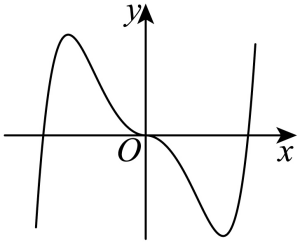
\includegraphics[width=4.6cm]{figures/2024_jiali_q7_A.png}}{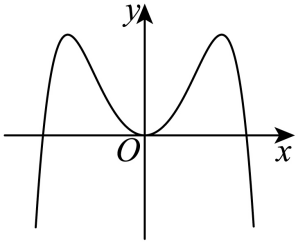
\includegraphics[width=4.6cm]{figures/2024_jiali_q7_B.png}}{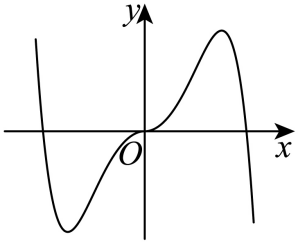
\includegraphics[width=4.6cm]{figures/2024_jiali_q7_C.png}}{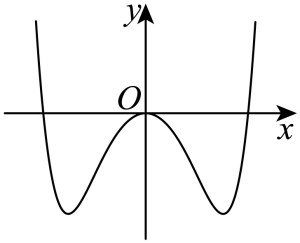
\includegraphics[width=4.6cm]{figures/2024_jiali_q7_D.png}}

\item 已知 $\dfrac{\cos\alpha}{\cos\alpha-\sin\alpha}=\sqrt3$，则 $\tan\left(\alpha+\dfrac{\pi}{4}\right)=$
\fourchoices{$2\sqrt3+1$}{$2\sqrt3-1$}{\tallchoice{$\dfrac{\sqrt3}{2}$}}{$1-\sqrt3$}

\item 已知向量 $\vec a=(x+1,x),\vec b=(x,2)$，则
\onechoices{$``x=-3"$ 是 $``\vec a\perp\vec b"$ 的必要条件}{$``x=-3"$ 是 $``\vec a\parallel\vec b"$ 的必要条件}{$``x=0"$ 是 $``\vec a\perp\vec b"$ 的充分条件}{$``x=-1+\sqrt3"$ 是 $``\vec a\parallel\vec b"$ 的充分条件}

\item 设 $\alpha,\beta$ 是两个平面，$m,n$ 是两条直线，且 $\alpha\cap\beta=m$. 下列四个命题：
①若 $m\parallel n$，则 $n\parallel\alpha$ 或 $n\parallel\beta$；②若 $m\perp n$，则 $n\perp\alpha,n\perp\beta$；③若 $n\parallel\alpha$，且 $n\parallel\beta$，则 $m\parallel n$；④若 $n$ 与 $\alpha$ 和 $\beta$ 所成的角相等，则 $m\perp n$. 其中所有真命题的编号是
\fourchoices{①③}{②④}{①②③}{①③④}

\item 在 $\triangle ABC$ 中内角 $A,B,C$ 所对边分别为 $a,b,c$，若 $B=\dfrac{\pi}{3}$，$b^2=\dfrac94ac$，则 $\sin A+\sin C=$
\fourchoices{\tallchoice{$\dfrac32$}}{$\sqrt2$}{\tallchoice{$\dfrac{\sqrt7}{2}$}}{\tallchoice{$\dfrac{\sqrt3}{2}$}}

\item 已知 $b$ 是 $a,c$ 的等差中项，直线 $ax+by+c=0$ 与圆 $x^2+y^2+4y-1=0$ 交于 $A,B$ 两点，则 $|AB|$ 的最小值为
\fourchoices{$2$}{$3$}{$4$}{$2\sqrt5$}
\end{examquestions}

\examsection{二、填空题：本题共4小题，每小题5分，共20分. }
\begin{examquestions}[start=13]
\item $\left(\dfrac13+x\right)^{10}$ 的展开式中，各项系数的最大值是\blank. 
\item 已知甲、乙两个圆台上、下底面的半径均为 $r_1$ 和 $r_2$，母线长分别为 $2(r_2-r_1)$ 和 $3(r_2-r_1)$，则两个圆台的体积之比 $\dfrac{V_{\text{甲}}}{V_{\text{乙}}}=\blank$. 
\item 已知 $a>1$，$\dfrac{1}{\log_8a}-\dfrac{1}{\log_a4}=-\dfrac52$，则 $a=\blank$. 
\item 有6个相同的球，分别标有数字1、2、3、4、5、6，从中不放回地随机抽取3次，每次取1个球. 记 $m$ 为前两次取出的球上数字的平均值，$n$ 为取出的三个球上数字的平均值，则 $m$ 与 $n$ 差的绝对值不超过 $\dfrac12$ 的概率是\blank. 
\end{examquestions}

\examsection{三、解答题：共70分. 解答应写出文字说明、证明过程或演算步骤. 第17题～第21题为必考题，每个考题考生必须作答. 第22、23题为选考题，考生根据要求作答. }
\examsection{（一）必考题：共60分. }
\begin{examanswers}[start=17]
\item（12分）

某工厂进行生产线智能化升级改造，升级改造后，从该工厂甲、乙两个车间产品中随机抽取150件进行检验，数据如下：
\begin{tightcenter}
\begin{tabular}{|c|c|c|c|c|}
\hline & 优级品 & 合格品 & 不合格品 & 总计\\ \hline
甲车间 & 26 & 24 & 0 & 50\\ \hline
乙车间 & 70 & 28 & 2 & 100\\ \hline
总计 & 96 & 52 & 2 & 150\\ \hline
\end{tabular}
\end{tightcenter}
（1）填写如下列联表：
\begin{tightcenter}
\begin{tabular}{|c|c|c|}
\hline & 优级品 & 非优级品\\ \hline
甲车间 & & \\ \hline
乙车间 & & \\ \hline
\end{tabular}
\end{tightcenter}
能否有95\%的把握认为甲、乙两车间产品的优级品率存在差异？能否有99\%的把握认为甲、乙两车间产品的优级品率存在差异？

（2）已知升级改造前该工厂产品的优级品率 $p=0.5$，设 $\overline p$ 为升级改造后抽取的 $n$ 件产品的优级品率. 如果 $\overline p>p+1.65\sqrt{\dfrac{p(1-p)}{n}}$，则认为该工厂产品的优级品率提高了，根据抽取的150件产品的数据，能否认为生产线智能化升级改造后，该工厂产品的优级品率提高了？（$\sqrt{150}\approx12.247$）

附：$K^2=\dfrac{n(ad-bc)^2}{(a+b)(c+d)(a+c)(b+d)}$. 
\begin{tightcenter}
\begin{tabular}{|c|c|c|c|}
\hline $P(K^2\geq k)$ & 0.050 & 0.010 & 0.001\\ \hline
$k$ & 3.841 & 6.635 & 10.828\\ \hline
\end{tabular}
\end{tightcenter}

\item（12分）

记 $S_n$ 为数列 $\{a_n\}$ 的前 $n$ 项和，且 $4S_n=3a_n+4$. 

（1）求 $\{a_n\}$ 的通项公式；

（2）设 $b_n=(-1)^{n-1}na_n$，求数列 $\{b_n\}$ 的前 $n$ 项和为 $T_n$. 

\item（12分）

如图，在以 $A,B,C,D,E,F$ 为顶点的五面体中，四边形 $ABCD$ 与四边形 $ADEF$ 均为等腰梯形，$BC\parallel AD,EF\parallel AD$，$AD=4,AB=BC=EF=2$，$ED=\sqrt{10},FB=2\sqrt3$，$M$ 为 $AD$ 的中点. 

\noindent\begin{minipage}[t]{0.64\linewidth}
（1）证明：$BM\parallel$ 平面 $CDE$；

（2）求二面角 $F-BM-E$ 的正弦值. 
\end{minipage}\hfill
\begin{minipage}[t]{0.30\linewidth}
\vspace{-1em}
\centering
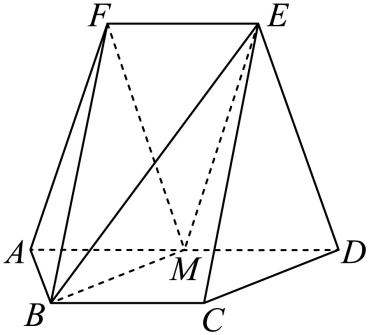
\includegraphics[width=\linewidth]{figures/2024_jiali_q19.png}
\end{minipage}

\item（12分）

设椭圆 $C:\dfrac{x^2}{a^2}+\dfrac{y^2}{b^2}=1(a>b>0)$ 的右焦点为 $F$，点 $M\left(1,\dfrac32\right)$ 在 $C$ 上，且 $MF\perp x$ 轴. 

（1）求 $C$ 的方程；

（2）过点 $P(4,0)$ 的直线与 $C$ 交于 $A,B$ 两点，$N$ 为线段 $FP$ 的中点，直线 $NB$ 交直线 $MF$ 于点 $Q$，证明：$AQ\perp y$ 轴. 

\item（12分）

已知函数 $f(x)=(1-ax)\ln(1+x)-x$. 

（1）当 $a=-2$ 时，求 $f(x)$ 的极值；

（2）当 $x\geq0$ 时，$f(x)\geq0$ 恒成立，求 $a$ 的取值范围. 
\end{examanswers}

\examsection{（二）选考题：共10分，请考生在第22、23题中任选一题作答，并用2B铅笔将所选题号涂黑，多涂、错涂、漏涂均不给分，如果多做，则按所做的第一题计分. }
\begin{examanswers}[start=22]
\item（10分）【选修4-4：坐标系与参数方程】

在平面直角坐标系 $xOy$ 中，以坐标原点 $O$ 为极点，$x$ 轴的正半轴为极轴建立极坐标系，曲线 $C$ 的极坐标方程为 $\rho=\rho\cos\theta+1$. 

（1）写出 $C$ 的直角坐标方程；

（2）设直线 $l:$\linsys{x=t,\\y=t+a}（$t$ 为参数），若 $C$ 与 $l$ 相交于 $A,B$ 两点，若 $|AB|=2$，求 $a$ 的值. 

\item（10分）【选修4-5：不等式选讲】

实数 $a,b$ 满足 $a+b\geq3$. 

（1）证明：$2a^2+2b^2>a+b$；

（2）证明：$|a-2b^2|+|b-2a^2|\geq6$. 
\end{examanswers}

\end{document}
